% =====================================================================
%  Chapitre 4 -- Entrainement, applications, projet
%  Partie a : teacher forcing, troncature, courbes
% =====================================================================
\section{Chapitre 4 --- Entraînement et applications}

\chapterslide{Chapitre 4}{Entraînement, applications et projet}%
{5 h --- teacher forcing, troncature, évaluation, projet}%
{\textbf{Objectifs.} Employer le teacher forcing et savoir pourquoi ; tronquer la
rétropropagation ; évaluer une prédiction sans fuite temporelle ; mener le projet
du module de bout en bout.}

\begin{frame}{Teacher forcing : apprendre vite, évaluer autrement}
\begin{center}
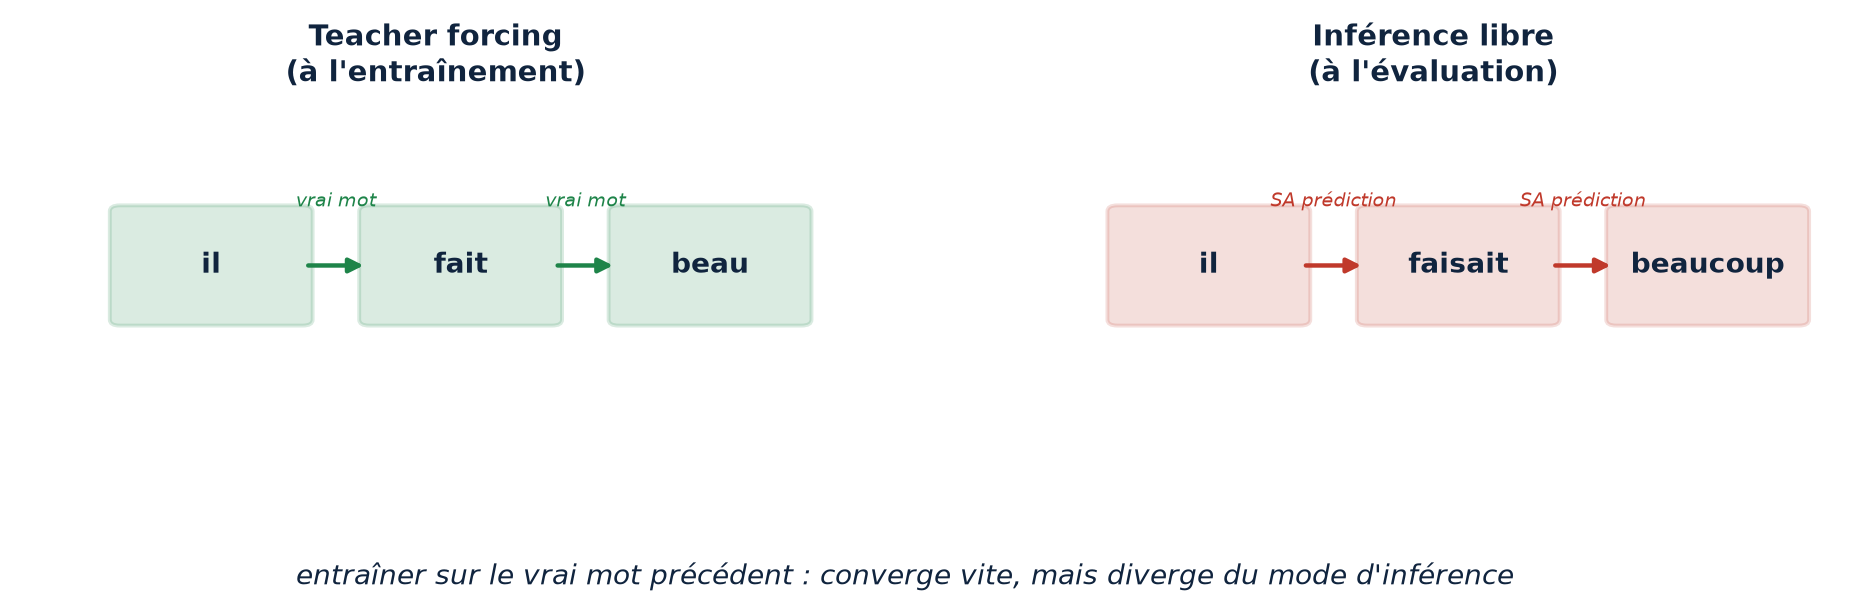
\includegraphics[width=0.92\textwidth]{u01_teacher_forcing.png}
\end{center}
\vspace{1mm}
\begin{columns}[t]
\begin{column}{0.48\textwidth}
\begin{solbox}[À l'entraînement]
On donne au décodeur le \textbf{vrai} mot précédent : le signal d'apprentissage
est propre et l'entraînement converge vite.
\end{solbox}
\end{column}
\begin{column}{0.48\textwidth}
\begin{wbox}[À l'évaluation]
Le vrai mot n'existe pas : le décodeur doit consommer \textbf{ses propres}
prédictions. L'écart entre les deux régimes s'appelle l'\textbf{exposure bias}.
\end{wbox}
\end{column}
\end{columns}
\end{frame}

\begin{frame}{Tronquer la rétropropagation}
\begin{center}
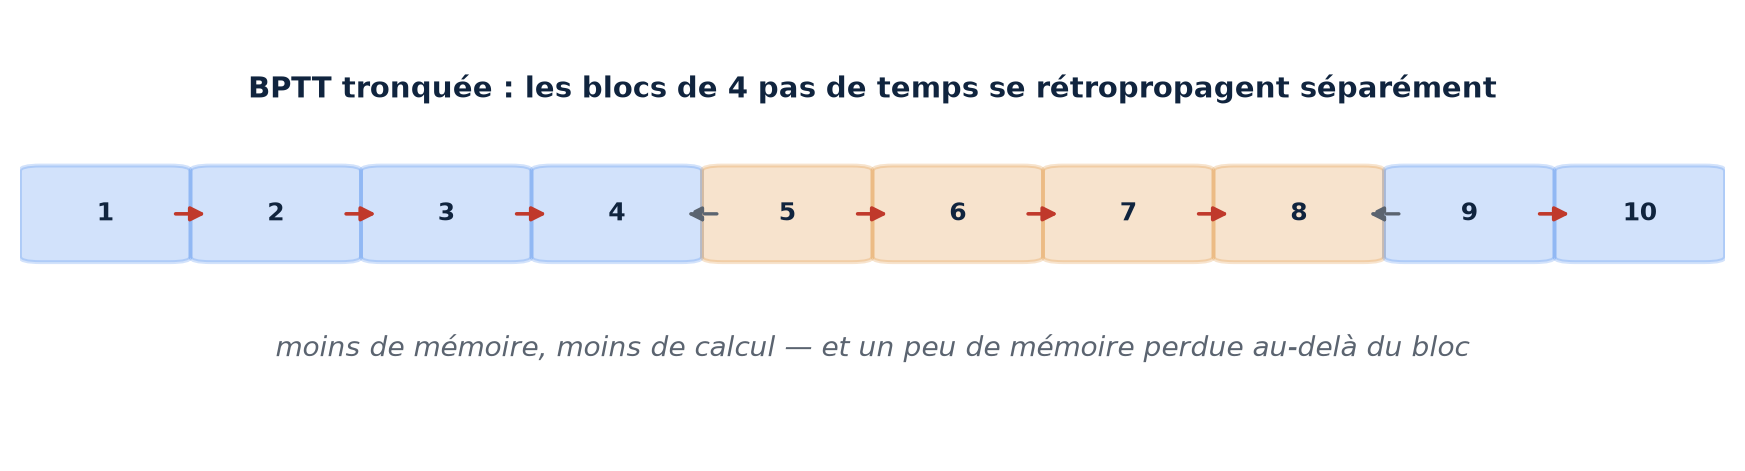
\includegraphics[width=0.94\textwidth]{u02_bptt_tronquee.png}
\end{center}
\vspace{1mm}
\begin{itemize}
  \item BPTT complète sur 500 pas : mémoire et temps de calcul énormes.
  \item On rétropropage par \textbf{blocs} de $k$ pas (ici $k = 4$) et on
  porte l'état caché d'un bloc au suivant.
\end{itemize}
\begin{kbox}[Le compromis]
$k$ trop petit : le réseau n'apprend pas les dépendances longues.
$k$ trop grand : coût de mémoire. En pratique : 20 à 200 pas selon la tâche.
\end{kbox}
\end{frame}

\begin{frame}{Ce que donne un LSTM bien entraîné}
\begin{center}
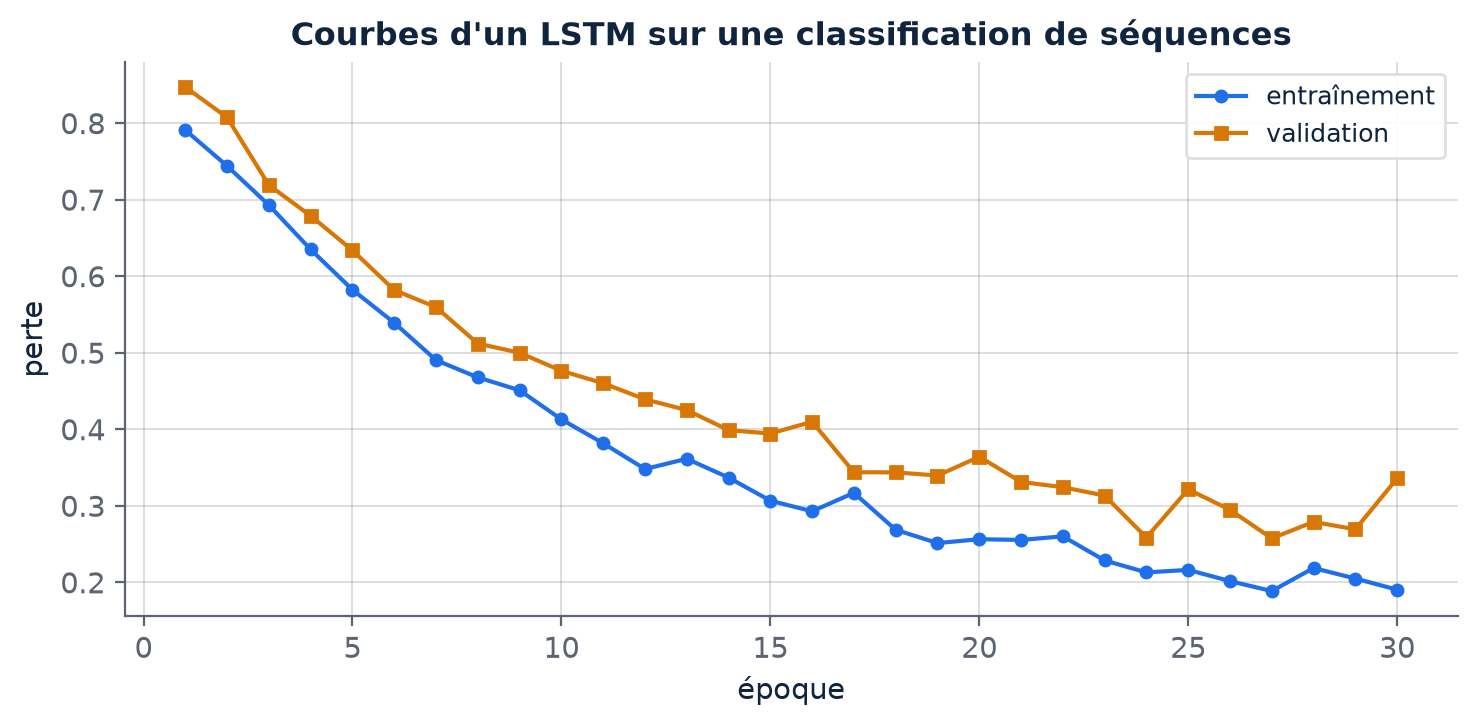
\includegraphics[width=0.8\textwidth]{u03_courbes.png}
\end{center}
\vspace{1mm}
\begin{kbox}[Lecture]
L'entraînement descend, la validation suit : le modèle apprend sans
surapprentissage visible. Un écart qui se creuse signale qu'il faut régulariser
(dropout sur les entrées et entre les couches récurrentes).
\end{kbox}
\end{frame}

\begin{frame}{Ce que chaque amélioration apporte}

\vspace{1mm}
\begin{itemize}
  \item Du RNN simple au LSTM : le gain de mémoire long terme (+5,7 points).
  \item Du LSTM au bidirectionnel : la double lecture (+3,5 points).
  \item Avec attention : encore +1,6 point.
\end{itemize}
\begin{wbox}[Ces valeurs sont un repère du cours]
Elles sortent d'une expérience exécutée (graine 4112) sur le jeu de données du
TP3 : ne les citez pas comme des constantes universelles.
\end{wbox}
% [fix] figure sortie
\end{frame}

\begin{frame}{Ce que chaque amélioration apporte --- la figure}\begin{center}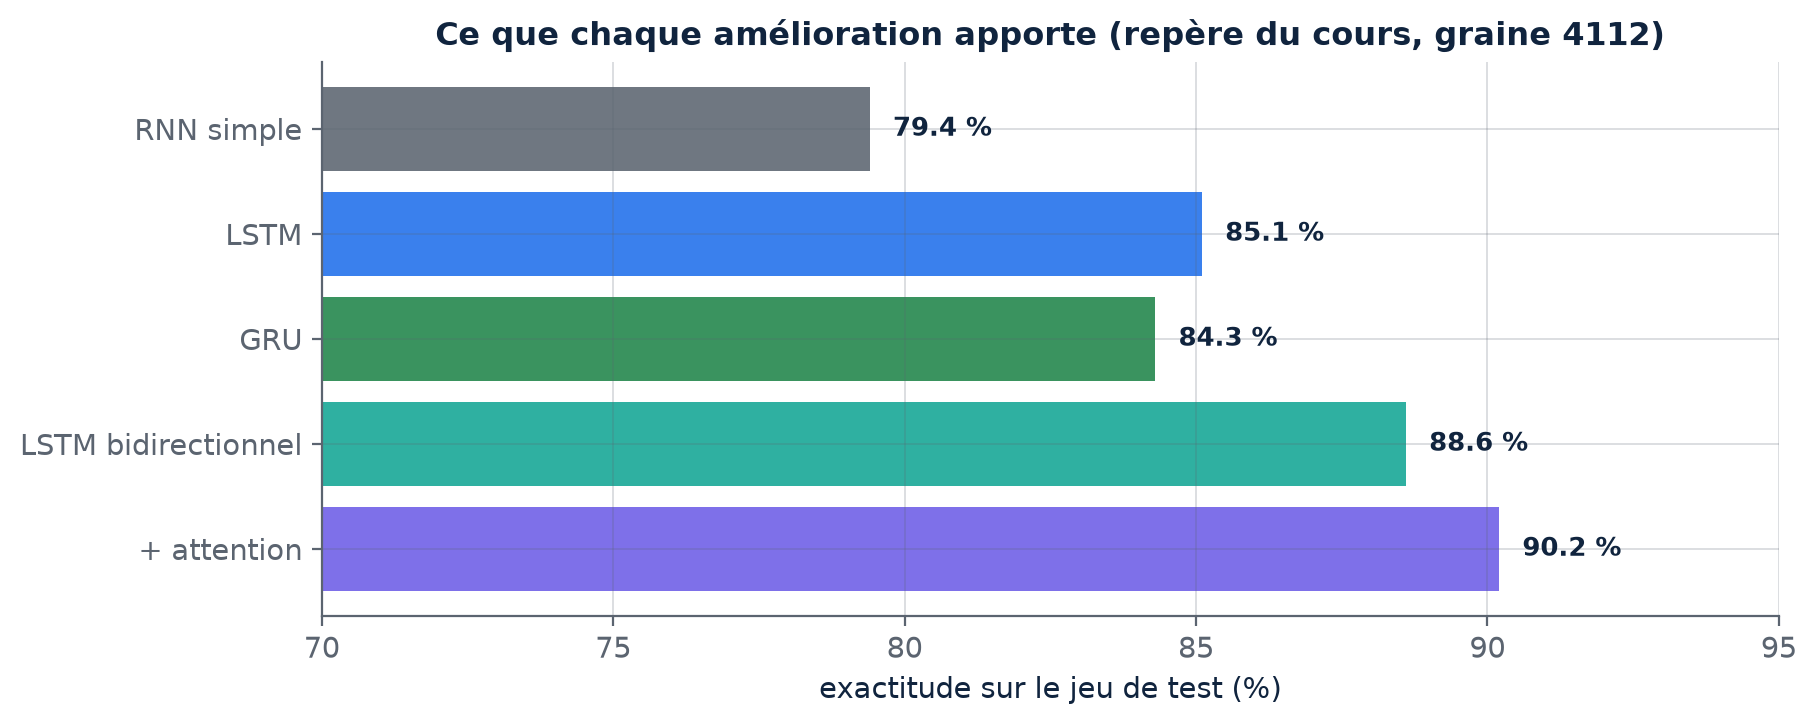
\includegraphics[width=.92\textwidth]{u04_comparaison.png}\end{center}\end{frame}

\begin{frame}{Prédire une série : le protocole honnête}
\begin{columns}[t]
\begin{column}{0.96\textwidth}
\begin{itemize}
  \item La série est \textbf{découpée dans le temps} : entraîner sur le passé,
  évaluer sur la suite.
  \item Le modèle ajusté ici est un AR-4 (moindres carrés) : ses coefficients
  sont calculés, pas inventés.
  \item RMSE mesuré sur l'horizon : \textbf{0{,}60}.
\end{itemize}
\begin{solbox}[Le geste professionnel]
Toujours comparer avec une \textbf{base de référence} triviale
(dernière valeur, moyenne glissante) avant de célébrer un RNN.
\end{solbox}
\end{column}
\end{columns}
% [fix] figure sortie
\end{frame}

\begin{frame}{Prédire une série : le protocole honnête --- la figure}\begin{center}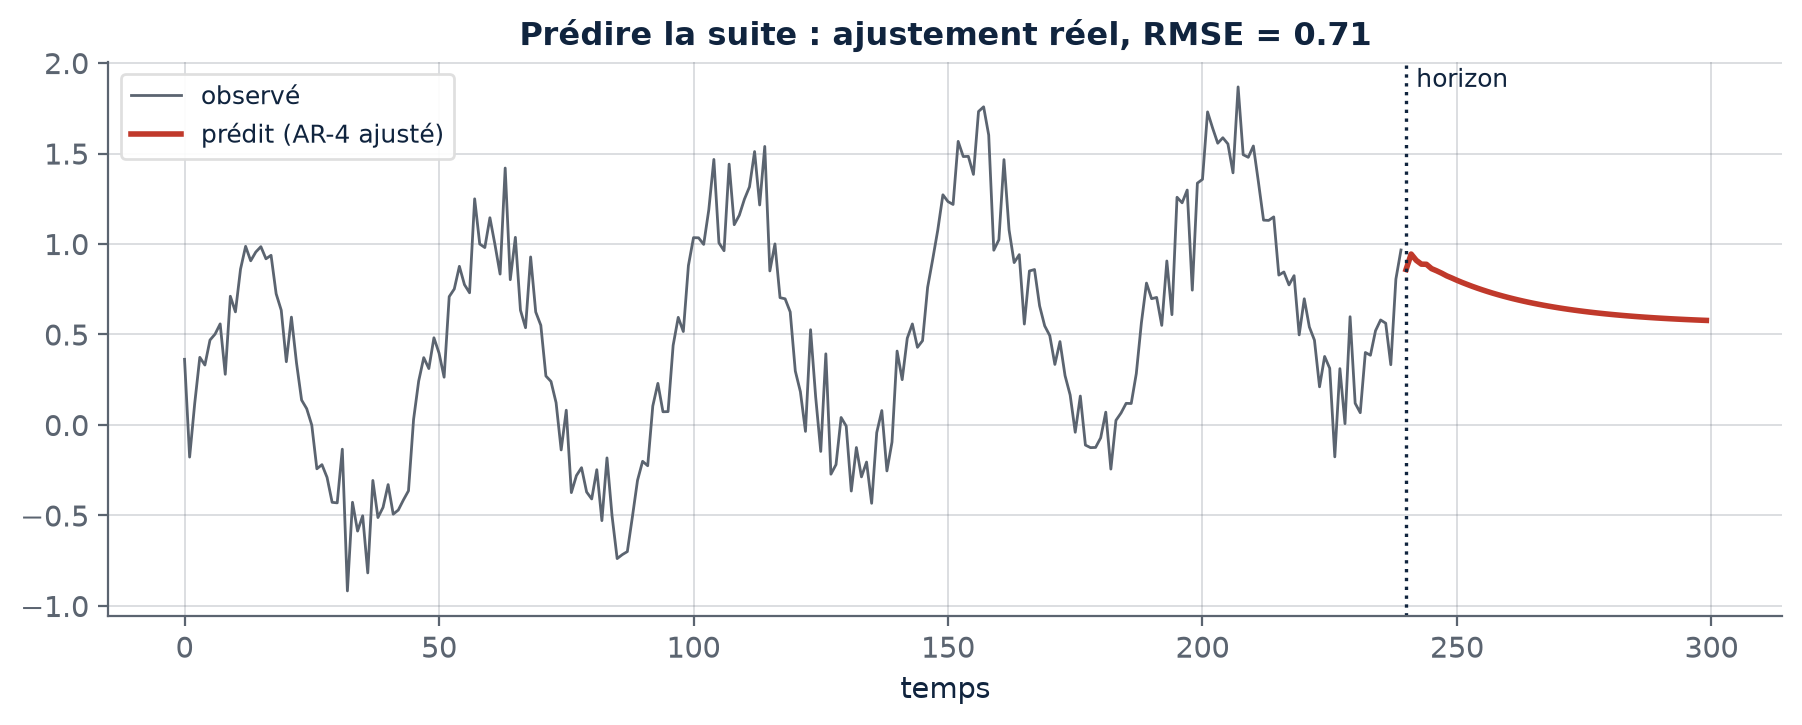
\includegraphics[width=.92\textwidth]{u05_prevision.png}\end{center}\end{frame}

\begin{frame}{Générer du texte : la température}
\begin{center}
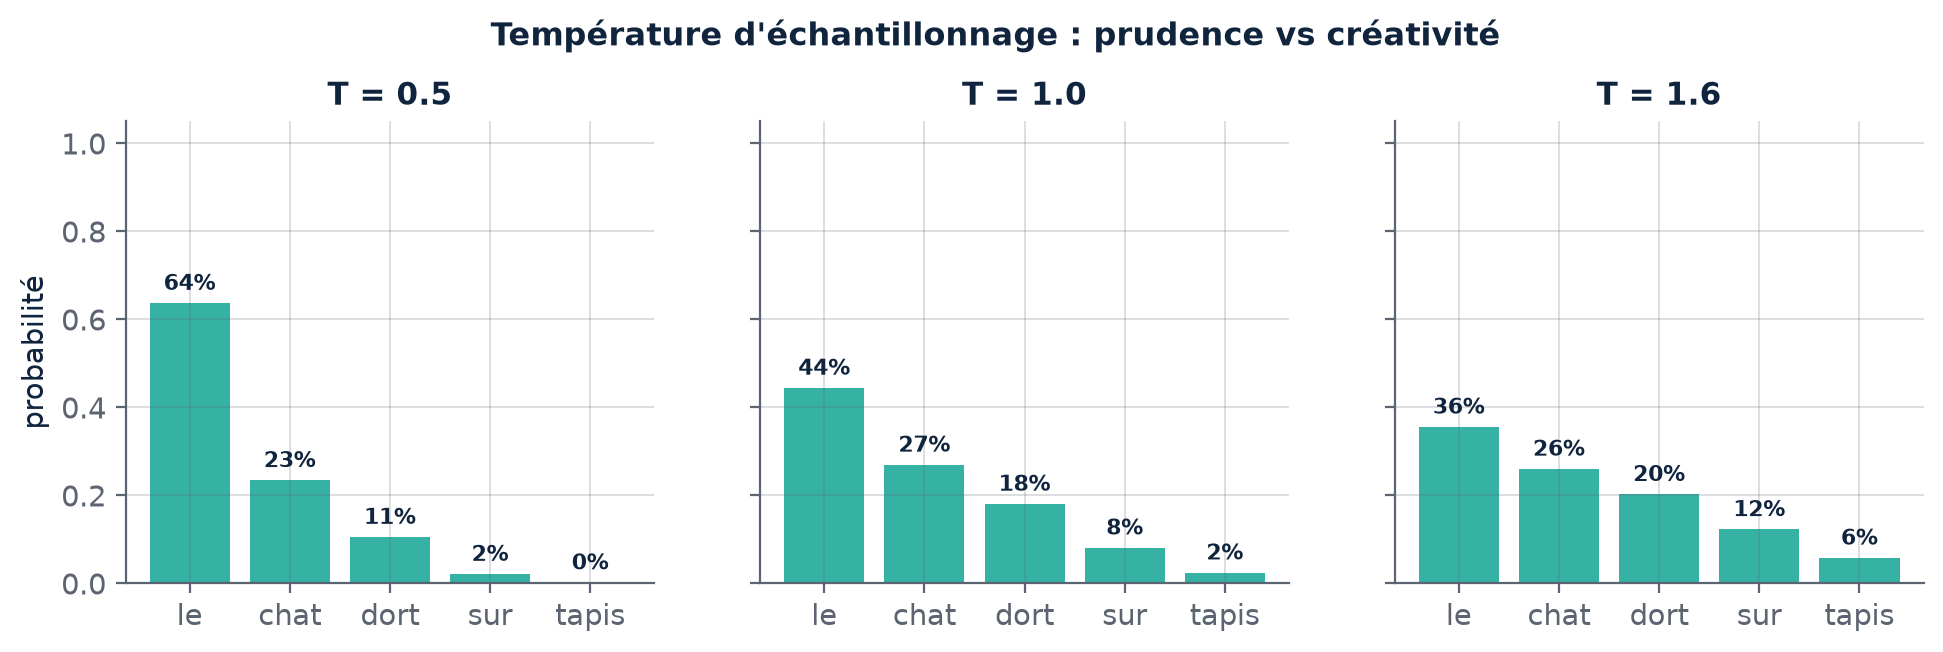
\includegraphics[width=0.9\textwidth]{u06_temperature.png}
\end{center}
\vspace{1mm}
\begin{itemize}
  \item $T < 1$ : la distribution se durcit --- prudent, répétitif.
  \item $T > 1$ : elle s'aplanit --- audacieux, incohérent.
  \item $T = 1$ : échantillonnage selon le modèle.
\end{itemize}
\end{frame}

\begin{frame}{Quiz 5 --- entraînement}
\begin{qbox}[Question 1]
Le teacher forcing consiste à nourrir le décodeur avec :
\begin{itemize}
  \item[(a)] ses propres prédictions \quad (b) le vrai mot précédent
  \quad (c) un vecteur nul
\end{itemize}
\end{qbox}
\begin{qbox}[Question 2]
La BPTT tronquée (blocs de $k$ pas) compromet…
\begin{itemize}
  \item[(a)] la mémoire et le calcul \quad (b) l'apprentissage des dépendances
  au-delà de $k$ \quad (c) la précision des poids
\end{itemize}
\end{qbox}
\begin{qbox}[Question 3]
Une température $T = 1{,}6$ produit un texte…
\begin{itemize}
  \item[(a)] plus prudent \quad (b) plus audacieux \quad (c) identique
\end{itemize}
\end{qbox}
\begin{solbox}[Réponses]
\textbf{1.} (b). \quad \textbf{2.} (b) : le gradient ne remonte pas au-delà du bloc. \quad
\textbf{3.} (b) : la distribution s'aplanit.
\end{solbox}
\end{frame}
